\section{Basic principals}\label{sec:basic_filter}

A digital filter is characterised as a \textit{linear time invariant} system referred to as a LTI system, which are to be described completely in the time domain by its impulse response $h[n]$. \\
When a discrete sequence $x[n]$ is applied to a LTI system it is the impulse response of the system $h[n]$ that determined what the output $y[n]$ will be. In other words the impulse response determine how much of the input sequence that passes the filter. \\ 
The output $y[n]$ is determined by the convolution sum of input signal and impulse response of the system.
\begin{align}
y[n] = x[n]*h[n] = \sum_{k=1}^{\infty} x[k]h[n-k]
\end{align}    
The frequency response of the system is given by the Fourier transformation of the impulse response. Consider the input sequence $x[n]=e^{j\omega n}$ for $-\infty < n <\infty$, then the frequency response is defined as\trine{side (40) DTSP}
\begin{align}\label{eq:freq_res}
H(e^{j\omega})=\sum_{k=-\infty}^{\infty}h[k]e^{-j\omega k}
\end{align}
thus the outcome of the filter becomes 
\begin{align}
y[n]=H(e^{j\omega})e^{-j\omega n} \label{eq:filter_output}
\end{align} \trine{evt. indsæt relations til Z og transferfunction her, og ny overskrift}
By \eqref{eq:filter_output} it is seen that $H(e^{j\omega})$ describes the change in complex amplitude of a complex exponential input signal to a given frequency. $H(e^{j\omega})$ is in general complex and hence it can be expressed as
\begin{align}
H(e^{j\omega})=|H(e^{j\omega})|e^{j\measuredangle H(e^{j\omega})}
\end{align}  
where $|H(e^{j\omega})|$ and $e^{j\measuredangle H(e^{j\omega})}$ are the \textit{magnitude} and \textit{phase} response of the filter respectively, both real valued and $2\pi$-periodic.\\ 
If the frequency response of a filter is real it is said to have \textit{zero phase}, which is equivalent to the phase response only taking values that are integer multiples of $\pi$, resolving in a straight phase with zero slope.   Further if the frequency response can be written in the form 
\begin{align}\label{eq:lin_pha}
H(e^{j\omega})=A(e^{j\omega})e^{j(-\alpha\omega + j\beta)} 
\end{align}
where $\alpha$ and $\beta$ are constants and $A(e^{j\omega})$ is real, the filter is said to have \textit{general linear phase}. That is because the phase response consist of constant terms added to the linear function making a straight line with slope $\alpha$ except from the discontinuities resolving from jumps of $2\pi$\trine{explain the discontinuity} \\
A linear phase response is characterized by a constant group delay $\tau(\omega)$
\begin{align}
\tau(\omega)=-\frac{d}{d\omega}\left\{ arg \left[ H(\text{e}^{j\omega}\right] \right\} = \alpha
\end{align}
The phase response is an expression of how each of the signal components are delayed though the system, where linear phase indicates an equal delay for all components of the signal. To guarantee a constant group delay, $\alpha$, $\beta$ and $h[n]$ has to fulfil the following condition, for all $\omega$
\begin{align}\label{eq:cons_gro}
\sum_{n=-\infty}^{\infty}h[n]\sin\left(\omega \left(n-\alpha \right) + \beta \right) = 0
\end{align}


\section{Ideal filters} 
When designing filters it is ideal to have approximately constant magnitude and zero phase corresponding to the frequency response. \\ For an ideal selective frequency filter the magnitude response will be constant unity for the frequencies that are wanted to pass the filter referred to as the \textit{bandpass} and zero for all other frequencies referred to as \textit{bandstop}. An example is an ideal lowpass filter with frequency response 
\begin{align}\label{eq:low}
H_{lp}(\text{e}^{j\omega})=
\left\{ \begin{matrix}
1, &\ \left| \omega \right|< \omega_c \\
0, &\ \omega_c < \left| \omega \right| \leq \pi
\end{matrix}\right.
\end{align}     
where $H_{lp}(\text{e}^{j\omega})$ is $2\pi$ periodic. $\omega_c$ is referred to as the \textit{cutoff frequency}. The lowpass filter selects the frequencies lower than the cutoff frequency and reject the higher frequency components of the signal. By \eqref{eq:low} it is seen that the lowpass filter is real valued hence has zero phase as expected. \\
The corresponding impulse response are determined by using the inverse Fourier transformation on the passband interval.
\begin{align}\label{eq:low_im}
h_{lp}[n]=\frac{1}{2\pi}\int_{-\omega_c}^{\omega_c}\text{e}^{j\omega n} d\omega = \frac{1}{2\pi j n}\left[\text{e}^{j\omega n} \right]_{-\omega_c}^{\omega_c} = \frac{\sin \omega_c n}{\pi n }, \ \  -\infty < n < \infty
\end{align}  
A system is called causal if the system output at time index \textit{k} depends only on input up to time \textit{k}. Further this implies $h[k] = 0$ for all $k<0$.\cite{FSP,p.196 & 208}  \\
By \eqref{eq:low_im} the impulse response is nonzero for $n<0$ hence the filter is noncasual.\\
Frequency- and impulse response are illustrated on figure \ref{?} \trine{Figur}
Analogues an ideal highpass or bandpass filter can be defined, as illustrated on figure \ref{fig:ideal}.\\ 

\begin{figure}[H]
	\begin{subfigure}[b]{0.32\textwidth}
        \centering

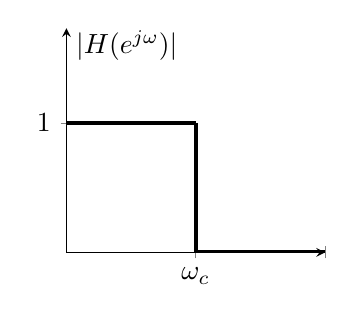
\begin{tikzpicture}[scale=1]
\begin{axis}[
scale=0.5,
unit vector ratio*=1 1 1,
axis lines = middle,
xtick={1.5,3},
xticklabels={$\omega_c$},
ytick={1.5},
yticklabels={$1$},
xmin=0,
xmax=3,
ymin=0,
ymax=2.6]
\node at (axis cs:0.7,2.4) {$|H(e^{j\omega})|$};
\draw[line width=0.5mm](axis cs:0,1.5)--(axis cs:1.5,1.5);
\draw[line width=0.5mm](axis cs:1.5,1.5)--(axis cs:1.5,0);
\draw[line width=0.5mm](axis cs:1.5,0)--(axis cs:3,0);
\end{axis}
\end{tikzpicture}
\caption{}
    \end{subfigure}
\begin{subfigure}[b]{0.32\textwidth}
        \centering

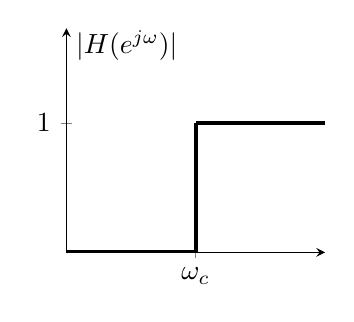
\begin{tikzpicture}[scale=1]
\begin{axis}[
scale=0.5,
unit vector ratio*=1 1 1,
axis lines = middle,
xtick={1.5},
xticklabels={$\omega_c$},
ytick={1.5},
yticklabels={$1$},
xmin=0,
xmax=3,
ymin=0,
ymax=2.6]
\node at (axis cs:0.7,2.4) {$|H(e^{j\omega})|$};
\draw[line width=0.5mm](axis cs:1.5,1.5)--(axis cs:3,1.5);
\draw[line width=0.5mm](axis cs:1.5,1.5)--(axis cs:1.5,0);
\draw[line width=0.5mm](axis cs:1.5,0)--(axis cs:0,0);
\end{axis}
\end{tikzpicture}

\caption{}
    \end{subfigure}
 \begin{subfigure}[b]{0.32\textwidth}
        \centering  
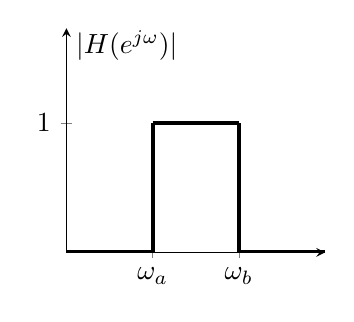
\begin{tikzpicture}[scale=1]
\begin{axis}[
scale=0.5,
unit vector ratio*=1 1 1,
axis lines = middle,
xtick={1,2},
xticklabels={$\omega_a$,$\omega_b$},
ytick={1.5},
yticklabels={$1$},
xmin=0,
xmax=3,
ymin=0,
ymax=2.6]
\node at (axis cs:0.7,2.4) {$|H(e^{j\omega})|$};
\draw[line width=0.5mm](axis cs:1,1.5)--(axis cs:1,0);
\draw[line width=0.5mm](axis cs:1,1.5)--(axis cs:2,1.5);
\draw[line width=0.5mm](axis cs:2,1.5)--(axis cs:2,0);
\draw[line width=0.5mm](axis cs:1,0)--(axis cs:0,0);
\draw[line width=0.5mm](axis cs:2,0)--(axis cs:3,0);
\end{axis}
\end{tikzpicture}
\caption{}
    \end{subfigure}
\caption{Magnitude of ideal (a) lowpass filter (b) highpass filter (c) bandpass filter}
\label{fig:ideal}
\end{figure}\trine{lav en figur med impuls responsen for a}
When computing a filter it is not possible to let the output depend on future input, hence noncausal systems are not computable, further zero phase is not possible for a causal system. 
Thus an approximation of an ideal filter can be computed by a casual system with general linear phase.    

\subsection{FIR and IIR filter} 
Two classes of filter are essential to identify.\\
For all ideal filters discussed in the previous section the impulse response is defined for $-\infty < n < \infty$ such filter is specified as a \textit{infinite impulse response (IIR)} filter . In the case of the impulse response being zero outside a finite interval the filter is referred to as a \textit{finit impulse response (FIR)} filter \\
\\
As described casual systems with generalized linear phase are wanted. This is possible to guaranty by using specific types of FIR filter.\\
A causal system with generalized linearphase has to fulfil the following relation, cf. section \ref{sec:basic_filter}
\begin{align}
\sum_{n=0}^{\infty}h[n]\sin\left(\omega \left(n-\alpha \right) + \beta \right) = 0
\end{align}
For a FIR filter to fulfil this relation the following set of conditions has to be fulfilled
\begin{align} \label{eq:FIR_con}
\beta = \left\{ \begin{matrix}
\pi  \\
0 
\end{matrix}\right. , \ \ 2\alpha = M = \text{an integer} , \ \ h[n]=h[M-n] \ \text{or} \ h[n]=-h[M-n]   
\end{align} 
this implies that $h[n]$ is either symmetric or anti symmetric and that $\alpha = \frac{M}{2}$ becomes the symmetric point. \\
On behave of these conditions four different types of FIR generalized linear phase filters is defined \cite{DTSP, p. 343}, only the type one filter will be elaborated here. Note that the conditions in \eqref{eq:FIR_con} guaranties a causal system with linear phase, but they are not a necessity. \\
A \textit{type 1 FIR filter} is characterised by having a symmetric impulse response and $M$ to be an even integer. By applying the the symmetry condition to the definition of the Fourier transformation the frequency response is defined by   
\begin{align}\label{eq:type1}
H(\text{e}^{j\omega})=\text{e}^{-j\omega \frac{M}{2}} \sum_{k=0}^{\frac{M}{2}} a[k]\cos \omega k
\end{align}
where 
\begin{align}
a[k]= \left\{ \begin{matrix}
2h\left[ \frac{M}{2} - k \right], \ \ &\ k=1,2,... , \frac{M}{2}.   \\
h[M-n], \ \ &\ k = 0  
\end{matrix}\right.
\end{align}
By this \eqref{eq:type1} has the form of\eqref{eq:lin_pha} where $A(\text{e}^{j\omega})= \sum_{k=0}^{\frac{M}{2}} a[k]\cos \omega k$ is a real function of $\omega$ and $\beta$ equals either 0 or $\pi$.\\
\\

sammenligning se side (510)DTSP
side (251)DTSP 






   
 


 



